\section{システム概要}
今回提案するシステムの全体を,図\ref{fig:structure_chart}に示す.
本システムでは,最初にPCワークを行うアプリケーション利用者(以下,ユーザ)が作業予定の設定を行う.
設定後,ユーザはアプリケーションを起動した状態のまま作業を行う.
その間,起動中のアプリケーションが,ユーザの作業状況を監視し,記録を行う.
記録された情報は,定期的に作業状況として監督者に通知され,監督者はユーザの行動を把握できる.

\begin{figure}[h]
  \begin{center}
  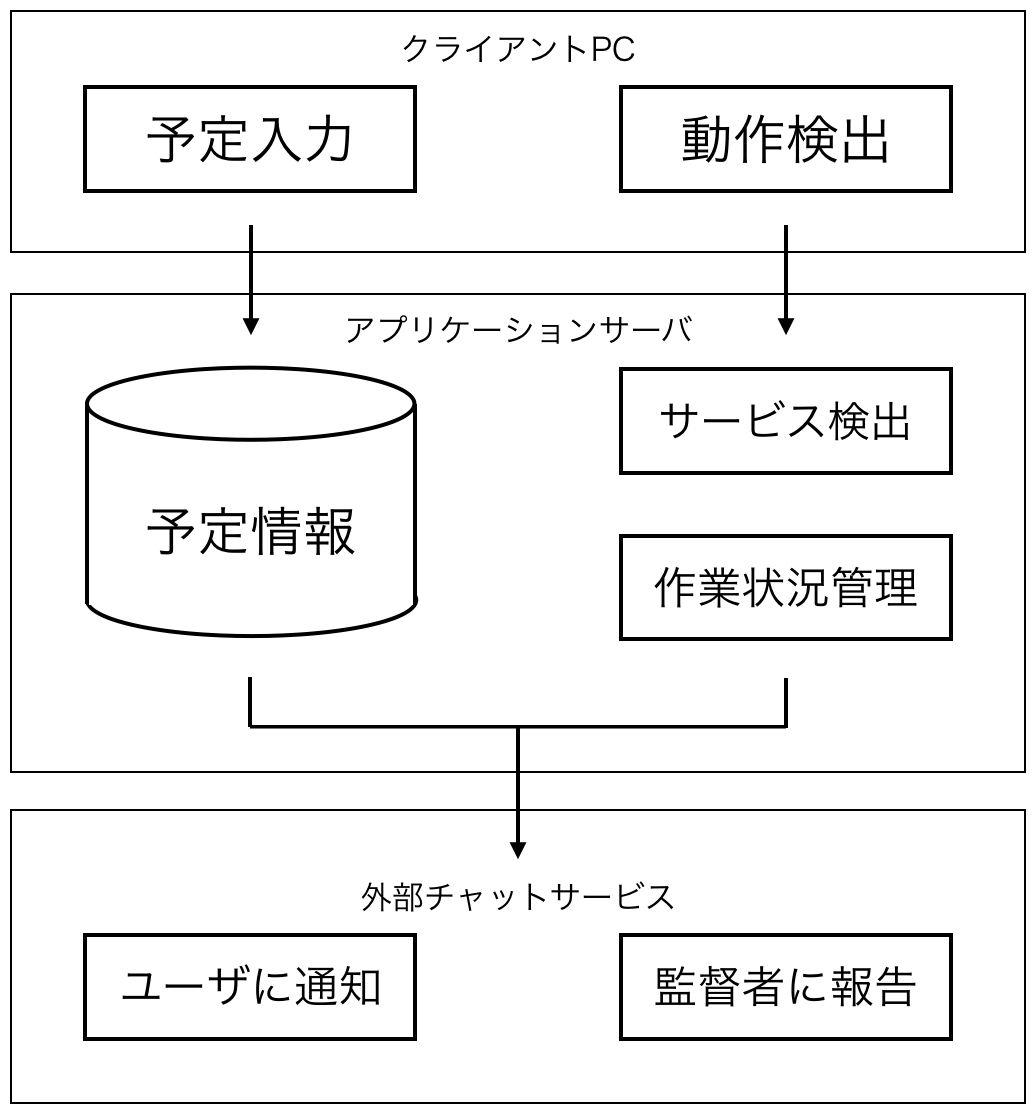
\includegraphics[width=8.0cm]{../graphics/structure_chart.png}
  \caption{システム構成図}
  \label{fig:structure_chart}
  \end{center}
\end{figure}
